\section{Experiments}

This sections contains experiments regarding the architecture of the variational autoencoder (VAE)
and the quality of the latent space. The experiments use the test and validation data of the RGB
imagery as well as the ground truth semantic labeling and the digital surface models as described in
\ref{datasets}.

\subsection{Variational Autoencoder Architecture} \label{architecture_experiments}

The experiments presented in this subsection determine the architecture that is used for the further
experiments regarding the latent space in the next subsection. All the tested VAE architectures have 
latent code of the size $1024$ and are trained with a batch size of $128$, $3000$ images over $50$ epochs.
This is done on the personal computer described in section \ref{hardware}.
The quality of the VAEs is on the one hand measured by the mean absolute error (MAE)
between the reconstruction and the input image.
On the other hand it is judged by the subjective opinion of how realistic the reconstructions look and how well
the semantic contents were recreated. This is the case since the MAE 
cannot capture the visual fidelity of a recreation. For instance if a reconstruction was an image that has the mean
color values of the input as every pixel it is just one color in all of the image and only one value was captured
from the input. However, this result has a lower MAE than an image with the inverted values of the
input. Clearly the inverted image is a much better reconstruction of the input than the unicolored image and therefore
additionally judging the results via a visual inspection is necessary.

The VAE architecture descriptions all cover an encoder up to a one dimensional tensor that is fed into two dense
layers which create the means and standard deviations as explained in section \ref{architecture}. Since these two
dense layers, the resampling and the dimension of the latent code is the same for every architecture the following
specifications of encoders do not include these features for brevity.
The inputs for every encoder are $128\times 128$ RGB images, i.e. $128\times 128\times 3$ images. The inputs
for every decoder are the latent code vectors of size $1,024$.


\subsubsection{Number of Convolutions} \label{section_number_of_convolutions_experiment}

This subsection contains 5 tests for which the encoder and decoder architectures are specified in Tables below.
The layers contained by the architecture in a test is specified by the number in the \textit{Test} column as 
described in the tables caption. This means that the test architecture $4$ has $6$ convolutional and
$6$ deconvolutional layers while test $1$ has only $3$ convolutional and $3$ deconvolutional
layers.

\begin{center}
    \begin{table}[H] \label{table_encoder_num_conv}
        \centering
        \begin{tabular}{ | c | l | c | }
            \multicolumn{3}{c}{Encoder} \\ \hline
            Test &Layer & Output\\ \hline
            all &Conv: Kernel $3\times3$, Stride $2\times2$, Filters $8  $    & $64\times 64\times 8  $    \\  
            all &Conv: Kernel $3\times3$, Stride $2\times2$, Filters $16 $    & $32\times 32\times 16 $    \\
            1   &Conv: Kernel $3\times3$, Stride $2\times2$, Filters $32 $    & $16\times 16\times 32 $    \\
            2   &Conv: Kernel $3\times3$, Stride $2\times2$, Filters $64 $    & $8\times 8\times   64 $    \\
            3   &Conv: Kernel $3\times3$, Stride $2\times2$, Filters $128$    & $4\times 4\times   128$    \\
            4   &Conv: Kernel $3\times3$, Stride $2\times2$, Filters $256$    & $2\times 2\times   256$    \\
            all &Flatten                                                              & $1,024$                    \\
            \hline
        \end{tabular} 
        \caption{The layers of the encoder of test $4$ up to the vector that the two dense layers use to produce 
        the means and standard deviations for the latent code. Test $x$ only contains the layers up to
        the layer with $x$ in the \textit{Test} column and the layers with \textit{all}.
        The output of the \textit{Flatten} layer
        varies depending on the test.}
    \end{table}
\end{center}
\vspace{-4em}
\begin{center}
    \begin{table}[H]
        \centering
        \begin{tabular}{ | c | l | c | }
            \multicolumn{3}{c}{Decoder} \\ \hline
            Test &Layer & Output\\ \hline
            all &Dense                                                            & $1,024$                   \\
            all &Reshape                                                          & $2\times 2\times    256$  \\
            4   &Deconv: Kernel $3\times3$, Stride $2\times2$, Filters $128$      & $4\times 4\times    128$  \\  
            3   &Deconv: Kernel $3\times3$, Stride $2\times2$, Filters $64 $      & $8\times 8\times    64 $  \\
            2   &Deconv: Kernel $3\times3$, Stride $2\times2$, Filters $32 $      & $16\times 16\times  32 $  \\
            1   &Deconv: Kernel $3\times3$, Stride $2\times2$, Filters $16 $      & $32\times 32\times  16 $  \\
            all &Deconv: Kernel $3\times3$, Stride $2\times2$, Filters $8  $      & $64\times 64\times  8  $  \\
            all &Deconv: Kernel $3\times3$, Stride $2\times2$, Filters $3  $      & $128\times 128\times3  $  \\
            \hline
        \end{tabular} 
        \caption{The layers of the decoder of test $4$. 
        Test $x$ only contains the layers after the layer with the number
        $x$ in the \textit{Test} column and the layers with \textit{all}.
        The outputs of the \textit{Dense} and \textit{Reshape}
        layers vary depending on the test.}
    \end{table}
\end{center}

\renewcommand{\thesubfigure}{\arabic{subfigure}}
\begin{figure}[H]
    \centering
    \begin{subfigure}{.25\textwidth}
        \centering
        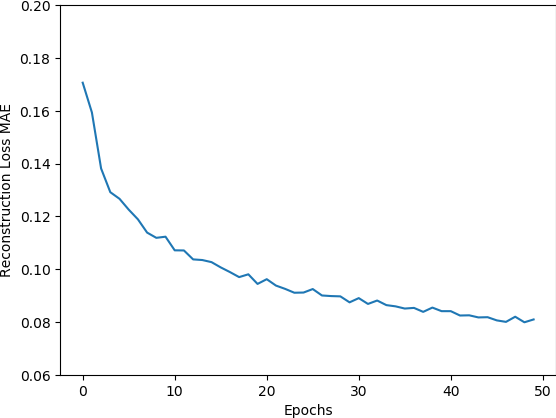
\includegraphics[width=\textwidth]
        {images/figures/experiments_architecture/mae_graphKernel3adjusted2x2x256_dim1024.png}
        \caption{}
    \end{subfigure}%
    \begin{subfigure}{.25\textwidth}
        \centering
        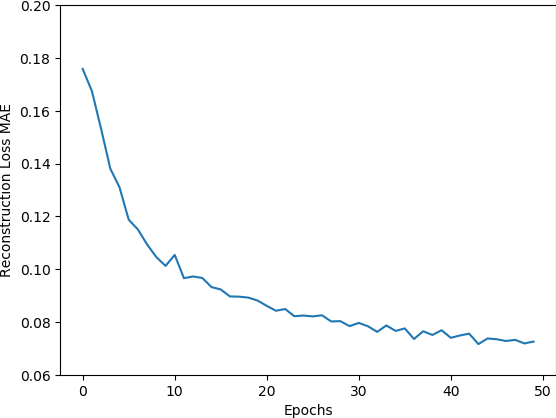
\includegraphics[width=\textwidth]
        {images/figures/experiments_architecture/mae_graphKernel3adjusted4x4x128_dim1024.png}
        \caption{}
    \end{subfigure}%
    \begin{subfigure}{.25\textwidth}
        \centering
        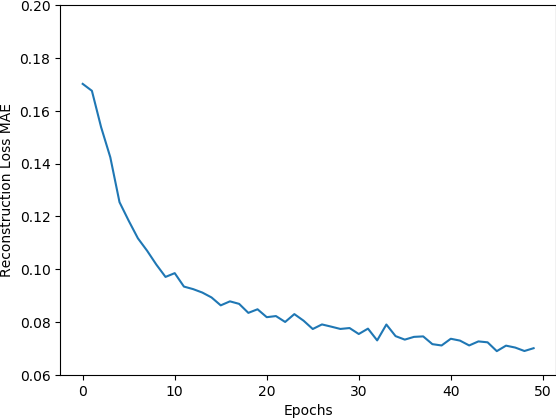
\includegraphics[width=\textwidth]
        {images/figures/experiments_architecture/mae_graphKernel3adjusted8x8x64_dim1024.png}
        \caption{}
    \end{subfigure}%
    \begin{subfigure}{.25\textwidth}
        \centering
        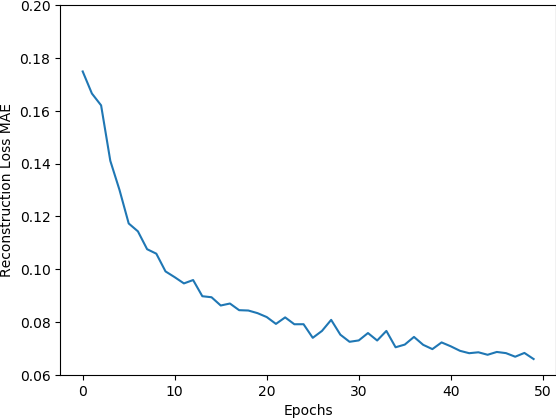
\includegraphics[width=\textwidth]
        {images/figures/experiments_architecture/mae_graphKernel3adjusted16x16x32_dim1024.png}
        \caption{}
    \end{subfigure}
    \caption{There is a graph for each test architecture.
    Each graph depicts the mean MAEs between input and reconstructions across all iterations in an epoch of training.}
\end{figure} \label{figure_learning_curves_1}

\begin{center}
    \begin{table}[H]
        \centering
        \begin{tabular}{ | c | c | c | c | }
            \hline
            Test &MAEs last Epoch & Loss last Epoch & Training time\\ \hline
            4 & $0.08093627$  & $0.08655346$  & 12 min 58 sec  \\
            3 & $0.07256235$  & $0.07953142$  & 13 min 17 sec  \\
            2 & $0.07004701$  & $0.07820769$  & 14 min 8 sec  \\  
            1 & $0.06594399$  & $0.0751977$  & 15 min 27 sec  \\  
            \hline
        \end{tabular} 
        \caption{For each test architecture the table shows the mean of the MAEs across all iterations of the last
        epoch, the mean loss across all iterations of the last epoch and the time it took to train the model
        on the personal computer as specified in section \ref{hardware}. Notice that the loss is not the same
        as MAE since it additionally takes the Kullback-Leibler divergence into account.}
    \end{table} \label{table_mae_1}
\end{center}


\begin{figure}[H] 
    \centering
    \begin{subfigure}[t]{.19\textwidth}
        \centering
        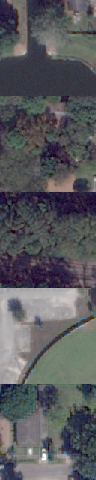
\includegraphics[width=0.5\textwidth]
        {images/figures/experiments_architecture/inputsCol1Kernel3adjusted32x32x32_dim1024.png}\hfill
        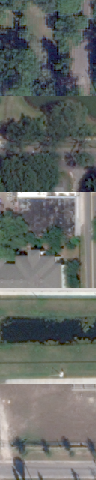
\includegraphics[width=0.5\textwidth]
        {images/figures/experiments_architecture/inputsCol2Kernel3adjusted32x32x32_dim1024.png}
    \end{subfigure}%
    \hspace*{0.1pt}
    \begin{subfigure}[t]{.19\textwidth}
        \centering
        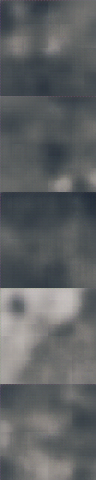
\includegraphics[width=0.5\textwidth]
        {images/figures/experiments_architecture/reconstructionsCol1Kernel3adjusted2x2x256_dim1024.png}\hfill
        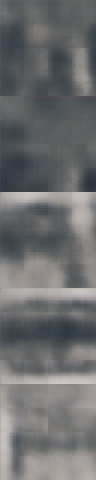
\includegraphics[width=0.5\textwidth]
        {images/figures/experiments_architecture/reconstructionsCol2Kernel3adjusted2x2x256_dim1024.png}
        \caption{}
    \end{subfigure}%
    \hspace*{0.1pt}
    \begin{subfigure}[t]{.19\textwidth}
        \centering
        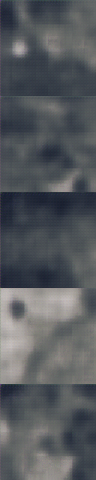
\includegraphics[width=0.5\textwidth]
        {images/figures/experiments_architecture/reconstructionsCol1Kernel3adjusted4x4x128_dim1024.png}\hfill
        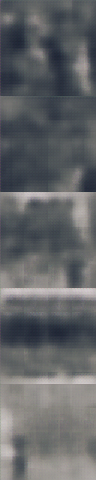
\includegraphics[width=0.5\textwidth]
        {images/figures/experiments_architecture/reconstructionsCol2Kernel3adjusted4x4x128_dim1024.png}
        \caption{}
    \end{subfigure}%
    \hspace*{0.1pt}
    \begin{subfigure}[t]{.19\textwidth}
        \centering
        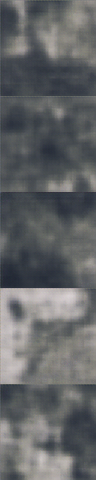
\includegraphics[width=0.5\textwidth]
        {images/figures/experiments_architecture/reconstructionsCol1Kernel3adjusted8x8x64_dim1024.png}\hfill
        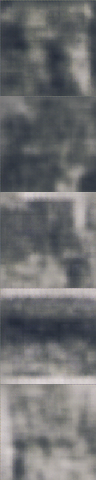
\includegraphics[width=0.5\textwidth]
        {images/figures/experiments_architecture/reconstructionsCol2Kernel3adjusted8x8x64_dim1024.png}
        \caption{}
    \end{subfigure}%
    \hspace*{0.1pt}
    \begin{subfigure}[t]{.19\textwidth}
        \centering
        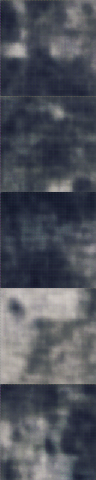
\includegraphics[width=0.5\textwidth]
        {images/figures/experiments_architecture/reconstructionsCol1Kernel3adjusted16x16x32_dim1024.png}\hfill
        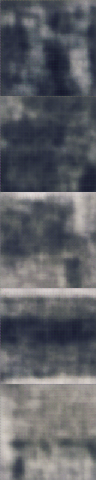
\includegraphics[width=0.5\textwidth]
        {images/figures/experiments_architecture/reconstructionsCol2Kernel3adjusted16x16x32_dim1024.png}
        \caption{}
    \end{subfigure}
    \caption{The left column shows original images taken from a validation set that the VAE has not seen during
    training. The other columns show the reconstructions of the VAE test architectures.}
\end{figure} \label{figure_reconstructions_1}

The learning curves in Figure \ref{figure_learning_curves_1} show a correlation between the MAE of the
reconstructions and the number of convolutional and deconvolutional layers. The less layers the are the better
is the learning curve which is in line with the visual fidelity of the reconstructions in Figure 
\ref{figure_reconstructions_1}. The reconstructions of the VAE with the least layers are the sharpest and the 
more layers the VAE has the blurrier the reconstructions are. 

A possible reason for this behavior is that the number of weights in the two dense layers between the 
last convolutional layer and the means and standard deviations increases drastically
if the number of convolutional layers decreases. This is the case because for each additional
value in the last convolutional layer there are $1,024$ additional weights in the three dense layers of the VAE
since $1,024$ is the size of the latent code. For example architecture $4$ only has $3,935,651$ weights while
architecture $3$, with one convolutional and deconvolutional layer less, has $6,492,192$ total weights.
The weights in the dense layers make up most of the total weights
and the higher amount of weights also leads to longer training times as it can be seen in Table \ref{table_mae_1}.
However, this increase in training time is negligible compared to the increase of the quality of the reconstructions. 

This leads to the idea that increasing the number of filters, and therefore the size of the dense layers, could yield
better results which is tested in the next section.



\subsubsection{Number of Filters} \label{section_number_of_filters}

The tables below describe test architectures in a similar way as the previous subsection 
\ref{section_number_of_convolutions_experiment}. The differences here are that the number of filters is doubled and
the last convolutional layer and the first deconvolutional layer is missing.

\begin{center}
    \begin{table}[H]
        \centering
        \begin{tabular}{ | c | l | c | }
            \multicolumn{3}{c}{Encoder} \\ \hline
            Include &Layer & Output\\ \hline
            all &Conv: Kernel $3\times3$, Stride $2\times2$, Filters $16 $    & $64\times 64\times 16 $    \\  
            1   &Conv: Kernel $3\times3$, Stride $2\times2$, Filters $32 $    & $32\times 32\times 32 $    \\
            2   &Conv: Kernel $3\times3$, Stride $2\times2$, Filters $64 $    & $16\times 16\times 64 $    \\
            3   &Conv: Kernel $3\times3$, Stride $2\times2$, Filters $128$    & $8\times 8\times   128$    \\
            4   &Conv: Kernel $3\times3$, Stride $2\times2$, Filters $256$    & $4\times 4\times   256$    \\
            all &Flatten                                                      & $2,048$                    \\
            \hline
        \end{tabular} 
        \caption{The layers of the encoder of test $4$ up to the vector that the two dense layers use to produce 
        the means and standard deviations for the latent code. Test $x$ only contains the layers up to
        the layer with $x$ in the \textit{Test} column and the layers with \textit{all}.
         The output of the \textit{Flatten} layer
        varies depending on the test.}
    \end{table}
\end{center}
\vspace{-4em}
\begin{center}
    \begin{table}[H]
        \centering
        \begin{tabular}{ | c | l | c | }
            \multicolumn{3}{c}{Decoder} \\ \hline
            Include &Layer & Output\\ \hline
            all &Dense                                                            & $2,048$                   \\
            all &Reshape                                                          & $4\times 4\times    256$  \\
            4   &Deconv: Kernel $3\times3$, Stride $2\times2$, Filters $128$      & $8\times 8\times    128$  \\
            3   &Deconv: Kernel $3\times3$, Stride $2\times2$, Filters $64 $      & $16\times 16\times  64 $  \\
            2   &Deconv: Kernel $3\times3$, Stride $2\times2$, Filters $32 $      & $32\times 32\times  32 $  \\
            1   &Deconv: Kernel $3\times3$, Stride $2\times2$, Filters $16 $      & $64\times 64\times  16 $  \\
            all &Deconv: Kernel $3\times3$, Stride $2\times2$, Filters $3  $      & $128\times 128\times3  $  \\
            \hline
        \end{tabular}
        \caption{The layers of the decoder of test $4$. 
        Test $x$ only contains the layers after the layer with the number
        $x$ in the \textit{Test} column and the layers with \textit{all}.
        The outputs of the \textit{Dense} and \textit{Reshape}
        layers vary depending on the test.} 
    \end{table}
\end{center}



\begin{figure}[H]
    \centering
    \begin{subfigure}{.25\textwidth}
        \centering
        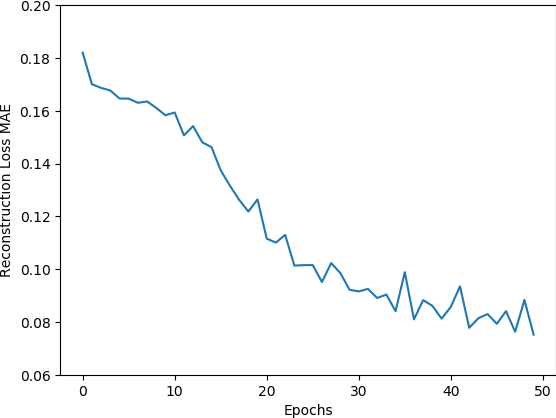
\includegraphics[width=\textwidth]
        {images/figures/experiments_architecture/mae_graphKernel3adjusted4x4x256_dim1024.png}
        \caption{}
    \end{subfigure}%
    \begin{subfigure}{.25\textwidth}
        \centering
        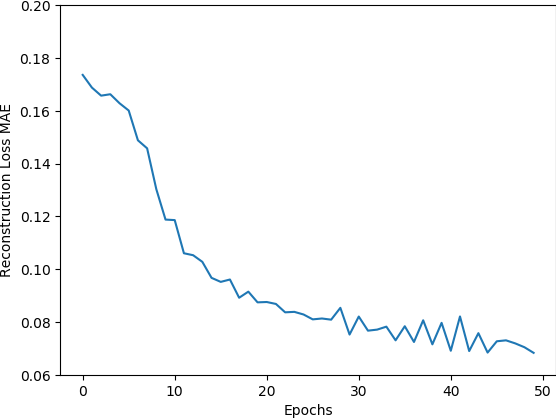
\includegraphics[width=\textwidth]
        {images/figures/experiments_architecture/mae_graphKernel3adjusted8x8x128_dim1024.png}
        \caption{}
    \end{subfigure}%
    \begin{subfigure}{.25\textwidth}
        \centering
        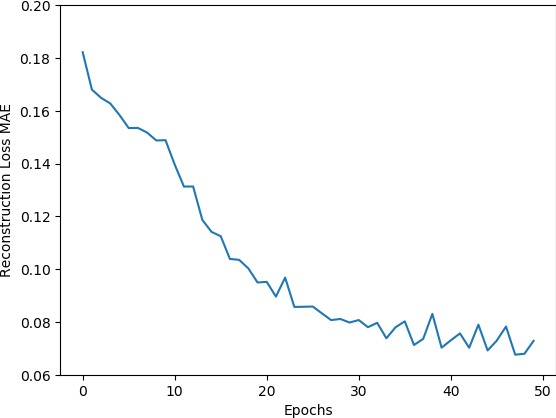
\includegraphics[width=\textwidth]
        {images/figures/experiments_architecture/mae_graphKernel3adjusted16x16x64_dim1024.png}
        \caption{}
    \end{subfigure}%
    \begin{subfigure}{.25\textwidth}
        \centering
        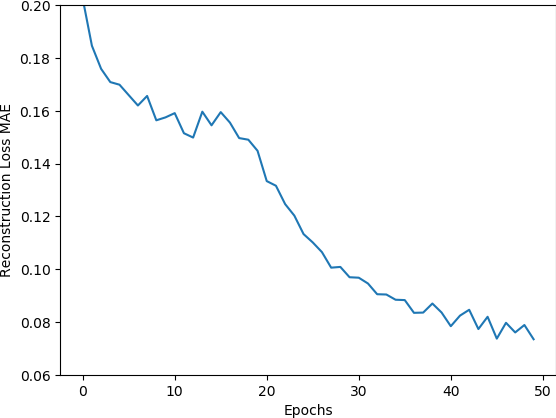
\includegraphics[width=\textwidth]
        {images/figures/experiments_architecture/mae_graphKernel3adjusted32x32x32_dim1024.png}
        \caption{}
    \end{subfigure}
    \caption{There is a graph for each test architecture.
    Each graph depicts the mean MAEs between input and reconstructions across all iterations in an epoch of training.}
\end{figure} \label{figure_learning_curves2}

\begin{center}
    \begin{table}[H]
        \centering
        \begin{tabular}{ | c | c | c | c | }
            \hline
            Test &MAEs last Epoch & Loss last Epoch & Training time\\ \hline
            4 & $0.07518449$  & $0.08227883$  & 21 min 31 sec  \\
            3 & $0.06828707$  & $0.07637741$  & 22 min 31 sec  \\
            2 & $0.07282908$  & $0.08208682$  & 26 min 17 sec  \\  
            1 & $0.07343805$  & $0.08214357$  & 34 min 31 sec  \\  
            \hline
        \end{tabular} 
        \caption{For each test architecture the table shows the mean of the MAEs across all iterations of the last
        epoch, the mean loss across all iterations of the last epoch and the time it took to train the model
        on the personal computer as described in section \ref{hardware}. Notice that the loss is not the same
        as MAE since it additionally takes the Kullback-Leibler divergence into account.}
    \end{table} \label{table_maes2}
\end{center}

\begin{figure}[H]
    \centering
    \begin{subfigure}[t]{.19\textwidth}
        \centering
        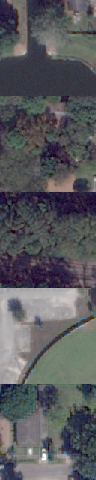
\includegraphics[width=0.5\textwidth]
        {images/figures/experiments_architecture/inputsCol1Kernel3adjusted32x32x32_dim1024.png}\hfill
        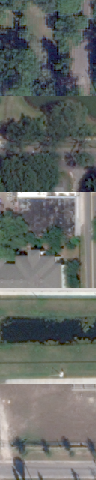
\includegraphics[width=0.5\textwidth]
        {images/figures/experiments_architecture/inputsCol2Kernel3adjusted32x32x32_dim1024.png}
    \end{subfigure}%
    \hspace*{0.1pt}
    \begin{subfigure}[t]{.19\textwidth}
        \centering
        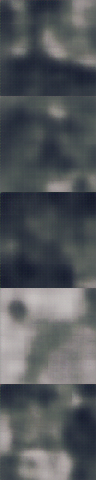
\includegraphics[width=0.5\textwidth]
        {images/figures/experiments_architecture/reconstructionsCol1Kernel3adjusted4x4x256_dim1024.png}\hfill
        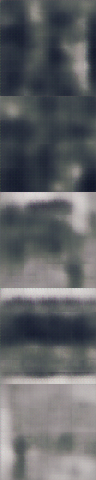
\includegraphics[width=0.5\textwidth]
        {images/figures/experiments_architecture/reconstructionsCol2Kernel3adjusted4x4x256_dim1024.png}
        \caption{}
    \end{subfigure}%
    \hspace*{0.1pt}
    \begin{subfigure}[t]{.19\textwidth}
        \centering
        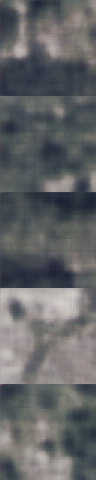
\includegraphics[width=0.5\textwidth]
        {images/figures/experiments_architecture/reconstructionsCol1Kernel3adjusted8x8x128_dim1024.png}\hfill
        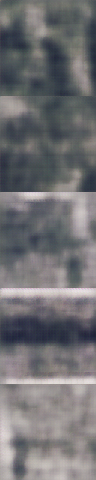
\includegraphics[width=0.5\textwidth]
        {images/figures/experiments_architecture/reconstructionsCol2Kernel3adjusted8x8x128_dim1024.png}
        \caption{}
    \end{subfigure}%
    \hspace*{0.1pt}
    \begin{subfigure}[t]{.19\textwidth}
        \centering
        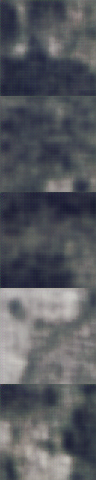
\includegraphics[width=0.5\textwidth]
        {images/figures/experiments_architecture/reconstructionsCol1Kernel3adjusted16x16x64_dim1024.png}\hfill
        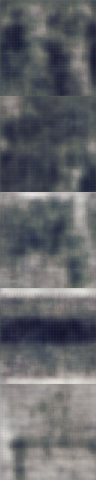
\includegraphics[width=0.5\textwidth]
        {images/figures/experiments_architecture/reconstructionsCol2Kernel3adjusted16x16x64_dim1024.png}
        \caption{}
    \end{subfigure}%
    \hspace*{0.1pt}
    \begin{subfigure}[t]{.19\textwidth}
        \centering
        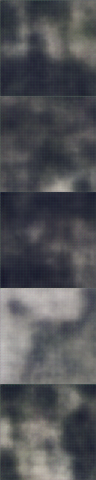
\includegraphics[width=0.5\textwidth]
        {images/figures/experiments_architecture/reconstructionsCol1Kernel3adjusted32x32x32_dim1024.png}\hfill
        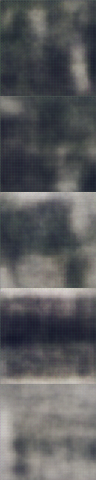
\includegraphics[width=0.5\textwidth]
        {images/figures/experiments_architecture/reconstructionsCol2Kernel3adjusted32x32x32_dim1024.png}
        \caption{}
    \end{subfigure}
    \caption{The left column shows original images taken from a validation set that the VAE has not seen during
    training. The other columns show the reconstructions of the VAE test architectures.}
\end{figure}

The trend of less layers correlating with better results does not hold up for the experiments in this subsection when
observing the MAEs in Table \ref{table_maes2}. However, the MAEs of the last epoch are not as crucial as in the 
previous subsection since the learning curves in Figure \ref{figure_learning_curves2} show a lot of variance in 
comparison to the previous subsection. Still the best MAE of the previous architectures beats all results of 
these tests while also taking less than halve as long to train and having more realistic looking reconstructions.


\subsubsection{Kernel Size}

In this subsection the two architectures $1$ and $3$, now called $1$ and $2$,
of the subsection \ref{section_number_of_convolutions_experiment}
are tested with a kernel size of $5\times 5$ instead of $3\times 3$. These architectures are chosen since architecture
$1$ performed the best so far and a second one is chosen for comparison. 

\begin{figure}[H]
    \centering
    \begin{subfigure}{.25\textwidth}
        \centering
        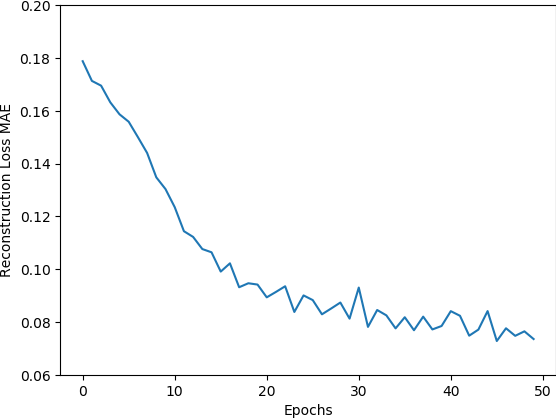
\includegraphics[width=\textwidth]
        {images/figures/experiments_architecture/mae_graphKernel5adjusted16x16x32_dim1024.png}
        \caption{}
    \end{subfigure}%
    \begin{subfigure}{.25\textwidth}
        \centering
        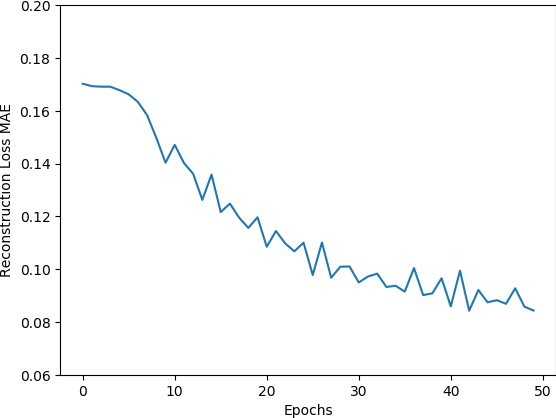
\includegraphics[width=\textwidth]
        {images/figures/experiments_architecture/mae_graphKernel5adjusted4x4x128_dim1024.png}
        \caption{}
    \end{subfigure}
    \caption{There is a graph for each test architecture.
    Each graph depicts the mean MAEs between input and reconstructions across all iterations in an epoch of training.}
\end{figure} \label{figure_learning_curves3}

\begin{center}
    \begin{table}[H]
        \centering
        \begin{tabular}{ | c | c | c | c | }
            \hline
            Test &MAEs last Epoch & Loss last Epoch & Training time\\ \hline
            2 & $0.08430038$  & $0.08984258$  & 19 min 19 sec  \\  
            1 & $0.07351803$  & $0.08184456$  & 19 min 40 sec  \\  
            \hline
        \end{tabular} 
        \caption{For each test architecture the table shows the mean of the MAEs across all iterations of the last
        epoch, the mean loss across all iterations of the last epoch and the time it took to train the model
        on the personal computer as described in section \ref{hardware}. Notice that the loss is not the same
        as MAE since it additionally takes the Kullback-Leibler divergence into account.}
    \end{table} \label{table_maes3}
\end{center}

\begin{figure}[H]
    \centering
    \begin{subfigure}[t]{.19\textwidth}
        \centering
        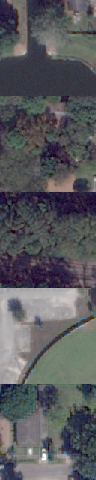
\includegraphics[width=0.5\textwidth]
        {images/figures/experiments_architecture/inputsCol1Kernel3adjusted32x32x32_dim1024.png}\hfill
        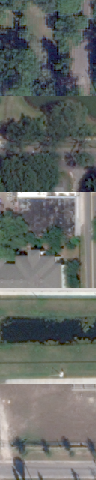
\includegraphics[width=0.5\textwidth]
        {images/figures/experiments_architecture/inputsCol2Kernel3adjusted32x32x32_dim1024.png}
    \end{subfigure}%
    \hspace*{0.1pt}
    \begin{subfigure}[t]{.19\textwidth}
        \centering
        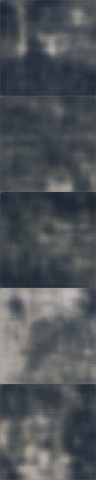
\includegraphics[width=0.5\textwidth]
        {images/figures/experiments_architecture/reconstructionsCol1Kernel5adjusted16x16x32_dim1024.png}\hfill
        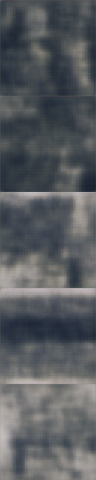
\includegraphics[width=0.5\textwidth]
        {images/figures/experiments_architecture/reconstructionsCol2Kernel5adjusted16x16x32_dim1024.png}
        \caption{}
    \end{subfigure}%
    \hspace*{0.1pt}
    \begin{subfigure}[t]{.19\textwidth}
        \centering
        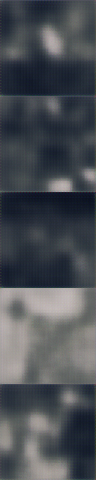
\includegraphics[width=0.5\textwidth]
        {images/figures/experiments_architecture/reconstructionsCol1Kernel5adjusted4x4x128_dim1024.png}\hfill
        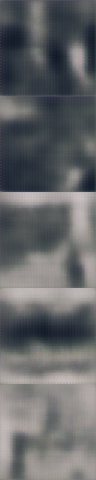
\includegraphics[width=0.5\textwidth]
        {images/figures/experiments_architecture/reconstructionsCol2Kernel5adjusted4x4x128_dim1024.png}
        \caption{}
    \end{subfigure}    
    \caption{The left column shows original images taken from a validation set that the VAE has not seen during
    training. The other columns show the reconstructions of the VAE test architectures.}
\end{figure}

The previously better performing architecture was better again with a higher kernel size. Still the results are 
all worse than those with the lower kernel size.

\subsubsection{Pooling}

This subsection tests the so far best performing architecture, number $1$ from subsection 
\ref{section_number_of_convolutions_experiment}, again but the convolutional layers now have a stride of $1\times1$
and the dimensionality reduction is done by pooling layers instead as visualized in the tables below. 
Additionally the architecture $2$ from subsection \ref{section_number_of_filters} is tested 
with similar modifications for comparison. The tests $1$ and $2$ refer to these architectures with max pooling
while $3$ and $4$ refer to the architectures with average pooling.

\begin{center}
    \begin{table}[H] \label{table_encoder_pooling}
        \centering
        \begin{tabular}{ | l | c | }
            \multicolumn{2}{c}{Encoder} \\ \hline
            Layer & Output\\ \hline
            Conv: Kernel $3\times3$, Stride $1\times1$, Filters $8  $    & $128\times 128\times 8  $    \\
            Pool: Pool size $2\times2$                                   & $64\times 64\times 8  $  \\
            Conv: Kernel $3\times3$, Stride $1\times1$, Filters $16 $    & $64\times 64\times 16 $    \\
            Pool: Pool size $2\times2$                                   & $32\times 32\times 16  $  \\
            Conv: Kernel $3\times3$, Stride $1\times1$, Filters $32 $    & $16\times 16\times 32 $    \\
            Pool: Pool size $2\times2$                                   & $16\times 16\times 32  $  \\
            Flatten                                                              & $1,024$            \\
            \hline
        \end{tabular} 
        \caption{The layers of the encoder of test $1$ up to the vector that the two dense layers use to produce 
        the means and standard deviations for the latent code.}
    \end{table}
\end{center}
\vspace{-4em}
\begin{center}
    \begin{table}[H]
        \centering
        \begin{tabular}{ | l | c | }
            \multicolumn{2}{c}{Decoder} \\ \hline
            Layer & Output\\ \hline
            Dense                                                            & $1,024$                   \\
            Reshape                                                          & $16\times 16\times  32 $  \\
            Deconv: Kernel $3\times3$, Stride $1\times1$, Filters $16 $      & $32\times 32\times  16 $  \\
            Deconv: Kernel $3\times3$, Stride $1\times1$, Filters $8  $      & $64\times 64\times  8  $  \\
            Deconv: Kernel $3\times3$, Stride $1\times1$, Filters $3  $      & $128\times 128\times3  $  \\
            \hline
        \end{tabular} 
        \caption{The layers of the decoder of test $1$.}
    \end{table}
\end{center}

\begin{figure}[H]
    \centering
    \begin{subfigure}{.25\textwidth}
        \centering
        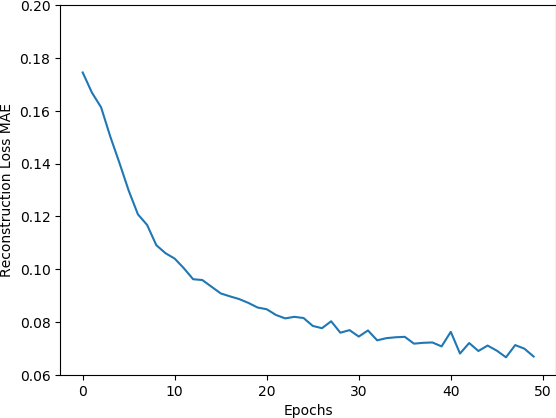
\includegraphics[width=\textwidth]
        {images/figures/experiments_architecture/mae_graphKernel3maxPool16x16x32_dim1024.png}
        \caption{}
    \end{subfigure}%
    \begin{subfigure}{.25\textwidth}
        \centering
        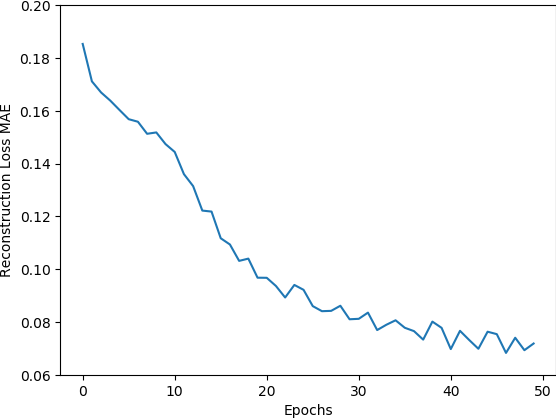
\includegraphics[width=\textwidth]
        {images/figures/experiments_architecture/mae_graphKernel3maxPool16x16x64_dim1024.png}
        \caption{}
    \end{subfigure}%
    \begin{subfigure}{.25\textwidth}
        \centering
        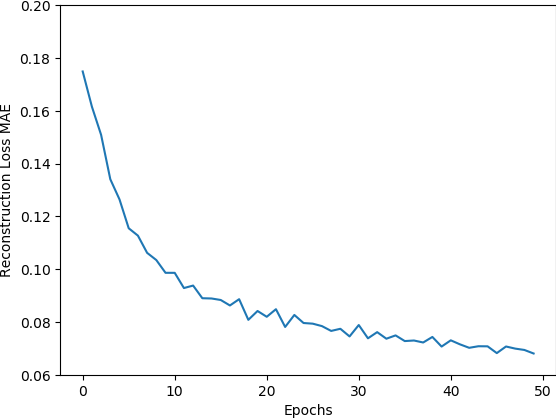
\includegraphics[width=\textwidth]
        {images/figures/experiments_architecture/mae_graphKernel3avgPool16x16x32_dim1024.png}
        \caption{}
    \end{subfigure}%
    \begin{subfigure}{.25\textwidth}
        \centering
        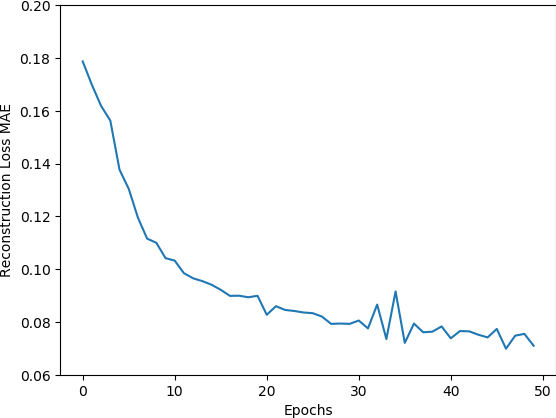
\includegraphics[width=\textwidth]
        {images/figures/experiments_architecture/mae_graphKernel3avgPool16x16x64_dim1024.png}
        \caption{}
    \end{subfigure}
    \caption{There is a graph for each test architecture.
    Each graph depicts the mean MAEs between input and reconstructions across all iterations in an epoch of training.}
\end{figure} \label{figure_learning_curves4}

\begin{center}
    \begin{table}[H]
        \centering
        \begin{tabular}{ | c | c | c | c | }
            \hline
            Test &MAEs last Epoch & Loss last Epoch & Training time\\ \hline
            4 & $0.07099171$  & $0.07931245$  & 53 min 11 sec  \\
            3 & $0.06803931$  & $0.07641139$  & 30 min 48 sec  \\
            2 & $0.07182192$  & $0.08001233$  & 54 min 9 sec  \\  
            1 & $0.06689975$  & $0.07499783$  & 31 min 39 sec  \\  
            \hline
        \end{tabular} 
        \caption{For each test architecture the table shows the mean of the MAEs across all iterations of the last
        epoch, the mean loss across all iterations of the last epoch and the time it took to train the model
        on the personal computer as described in section \ref{hardware}. Notice that the loss is not the same
        as MAE since it additionally takes the Kullback-Leibler divergence into account.}
    \end{table} \label{table_maes4}
\end{center}

\begin{figure}[H]
    \centering
    \begin{subfigure}[t]{.19\textwidth}
        \centering
        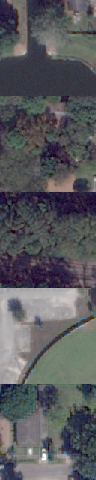
\includegraphics[width=0.5\textwidth]
        {images/figures/experiments_architecture/inputsCol1Kernel3adjusted32x32x32_dim1024.png}\hfill
        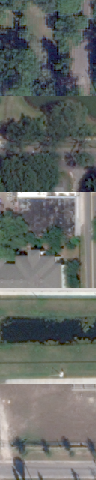
\includegraphics[width=0.5\textwidth]
        {images/figures/experiments_architecture/inputsCol2Kernel3adjusted32x32x32_dim1024.png}
    \end{subfigure}%
    \hspace*{0.1pt}
    \begin{subfigure}[t]{.19\textwidth}
        \centering
        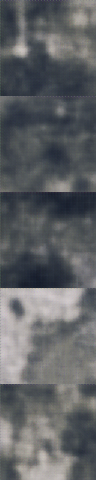
\includegraphics[width=0.5\textwidth]
        {images/figures/experiments_architecture/reconstructionsCol1Kernel3maxPool16x16x32_dim1024.png}\hfill
        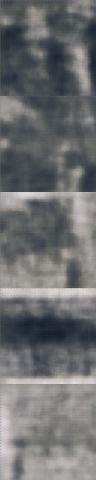
\includegraphics[width=0.5\textwidth]
        {images/figures/experiments_architecture/reconstructionsCol2Kernel3maxPool16x16x32_dim1024.png}
        \caption{}
    \end{subfigure}%
    \hspace*{0.1pt}
    \begin{subfigure}[t]{.19\textwidth}
        \centering
        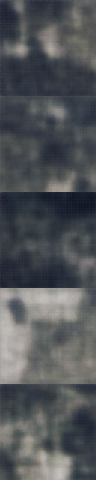
\includegraphics[width=0.5\textwidth]
        {images/figures/experiments_architecture/reconstructionsCol1Kernel3maxPool16x16x64_dim1024.png}\hfill
        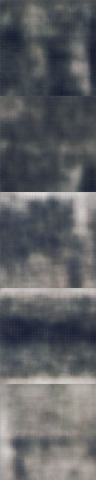
\includegraphics[width=0.5\textwidth]
        {images/figures/experiments_architecture/reconstructionsCol2Kernel3maxPool16x16x64_dim1024.png}
        \caption{}
    \end{subfigure}%
    \hspace*{0.1pt}
    \begin{subfigure}[t]{.19\textwidth}
        \centering
        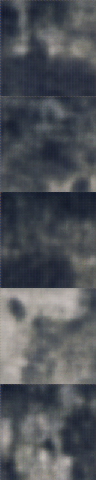
\includegraphics[width=0.5\textwidth]
        {images/figures/experiments_architecture/reconstructionsCol1Kernel3avgPool16x16x32_dim1024.png}\hfill
        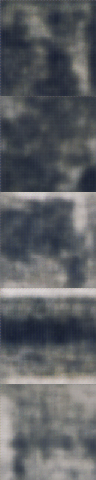
\includegraphics[width=0.5\textwidth]
        {images/figures/experiments_architecture/reconstructionsCol2Kernel3avgPool16x16x32_dim1024.png}
        \caption{}
    \end{subfigure}%
    \hspace*{0.1pt}
    \begin{subfigure}[t]{.19\textwidth}
        \centering
        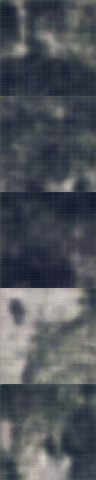
\includegraphics[width=0.5\textwidth]
        {images/figures/experiments_architecture/reconstructionsCol1Kernel3avgPool16x16x64_dim1024.png}\hfill
        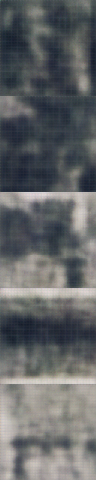
\includegraphics[width=0.5\textwidth]
        {images/figures/experiments_architecture/reconstructionsCol2Kernel3avgPool16x16x64_dim1024.png}
        \caption{}
    \end{subfigure}
    \caption{The left column shows original images taken from a validation set that the VAE has not seen during
    training. The other columns show the reconstructions of the VAE test architectures.}
\end{figure}

Regarding the results in Table \ref{table_maes4} it could be argued that pooling just led to worse results with
MAEs that are a bit worse and training times that are far longer. However, the visual fidelity of the recreations
is judged as the best for architecture $1$ of this subsection.


\subsubsection{Best Architectures}

The two architectures that came out as the best regarding visual fidelity and the MAE between inputs and 
reconstructions are number $1$ from subsection \ref{section_number_of_convolutions_experiment} and that architecture
with max pooling. These are also the architectures presented in section \ref{architecture} that are used
for the further experiments regarding the latent space. The following Figure \ref{figure_results_trained_on_all}
shows the reconstructions of these architectures trained on the full training set of $178,112$ images instead
of just $3000$ images. The size of the latent code is $1,024$ again.

As expected the reconstructions are a lot better and apart from a bit of blur they look the same as the originals.

\renewcommand{\thesubfigure}{\alph{subfigure}}
\begin{figure}[H]
    \centering
    \begin{subfigure}[t]{.19\textwidth}
        \centering
        \includegraphics[width=0.5\textwidth]
        {images/figures/experiments_architecture/inputsCol1Kernel3adjusted32x32x32_dim1024.png}\hfill
        \includegraphics[width=0.5\textwidth]
        {images/figures/experiments_architecture/inputsCol2Kernel3adjusted32x32x32_dim1024.png}
    \end{subfigure}%
    \hspace*{0.1pt}
    \begin{subfigure}[t]{.19\textwidth}
        \centering
        \includegraphics[width=0.5\textwidth]
        {images/figures/experiments_architecture/reconstructionsCol116x16x32TRAINEDON178000_dim1024.png}\hfill
        \includegraphics[width=0.5\textwidth]
        {images/figures/experiments_architecture/reconstructionsCol216x16x32TRAINEDON178000_dim1024.png}
        \caption{}
    \end{subfigure}%
    \hspace*{0.1pt}
    \begin{subfigure}[t]{.19\textwidth}
        \centering
        \includegraphics[width=0.5\textwidth]
        {images/figures/experiments_architecture/reconstructionsCol1Kernel3maxPool16x16x64_dim1024.png}\hfill
        \includegraphics[width=0.5\textwidth]
        {images/figures/experiments_architecture/reconstructionsCol2Kernel3maxPool16x16x64_dim1024.png}
        \caption{}
    \end{subfigure}
    \caption{The left column shows original images taken from a validation set that the VAE has not seen during
    training. Column $(a)$ shows the reconstructions of the fully convolutional VAE while column $(b)$ 
    depicts the reconstructions of the max pooling architecture.}
\end{figure} \label{figure_results_trained_on_all}


%TODO in the images above column b is still wrong and needs to be replaced with the actual images  

\subsection{Latent Space} \label{latent_space_experiments}
